\section{Why Recommendation Matters for Agent Memory}
\label{sec:memory-use}

We study recommendation as the step that turns stored memory into evidence for a current task.
Table~\ref{tab:recommendation-effect} isolates its contribution with context construction fixed, covering all six settings from three benchmark suites: RULER document QA and MQuAKE-derived FactConsolidation (FC) in MemoryAgentBench~\citep{hu2026memoryagentbench}, LoCoMo, and 2WikiMultiHopQA.
These four data origins contribute 3,386 questions in their full configured releases, including HippoRAG's 1,000-question 2Wiki subset.
We retain the native prompts and metrics and the main experiments' seed-42 development evaluation.
Four-reader results follow Qwen3.5-4B/Qwen3.5-9B/Gemma3-4B/Llama3.1-8B order.
Recommendation improves 22 of the 24 task--reader scores.
We investigate the task requirements behind these gains and the conversational exception.

\begin{table}[ht]
\centering
\small
\setlength{\tabcolsep}{3pt}
\begin{tabular}{lrrrr}
\toprule
Task ($n$) & Q4 & Q9 & G & L \\
\midrule
SH-Doc (100) & +9.0 & +11.0 & +10.0 & +8.0 \\
MH-Doc (100) & +13.0 & +13.0 & +9.0 & +15.0 \\
FC-SH (100) & +4.0 & +9.0 & +1.0 & +10.0 \\
FC-MH (100) & +9.0 & +12.0 & +6.0 & +5.0 \\
LoCoMo (1,986) & -1.9 & -0.5 & +0.5 & +0.4 \\
2Wiki (1,000) & +13.3 & +12.3 & +10.2 & +9.7 \\
\bottomrule
\end{tabular}
\caption{Effect of recommendation on native answer scores (percentage points), with context construction unchanged. The control replaces graph recommendation with dense selection and retains BM25 fusion. Document/FC scores are substring EM; 2Wiki is answer F1; LoCoMo uses its native category metrics.}
\label{tab:recommendation-effect}
\end{table}


\begin{figure*}[!t]
\centering
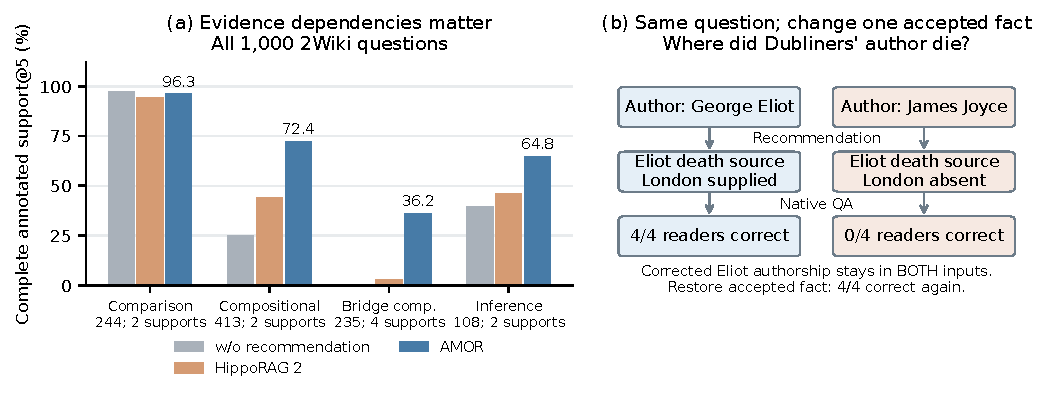
\includegraphics[width=\textwidth]{figures/memory_recommendation.pdf}
\caption{\textbf{Recommendation follows dependencies within memory.} (a) Official 2Wiki question types: comparison and compositional questions both require two supporting passages, but their response to recommendation differs substantially. Counts and support requirements appear below each type. (b) A source-verified FC-MH intervention. Only the accepted authorship changes; graph, matching confidence, and later processing stay fixed. The corrected authorship remains in both final inputs. Arrows show the observed selection/answer sequence, not a purported graph traversal path.}
\label{fig:memory-recommendation}
\end{figure*}

\begin{table*}[!t]
\centering
\small
\setlength{\tabcolsep}{4pt}
\begin{tabular}{>{\raggedright\arraybackslash}p{.17\textwidth}>{\raggedright\arraybackslash}p{.31\textwidth}>{\raggedright\arraybackslash}p{.29\textwidth}>{\raggedright\arraybackslash}p{.15\textwidth}}
\toprule
Question / data & Memory that identifies what is needed & Additional evidence and controlled change & Outcome \\
\midrule
Older film director?\newline 2Wiki & \emph{God's Gift to Women}: Michael Curtiz; other film: Edith Carlmar. Both directors are recognized. & Biographies give 1886 versus 1911. Change only Curtiz--biography weight $26\to1$; restore on unit graph. & Complete support $4/4\to3/4\to4/4$. \\
\addlinespace[3pt]
\emph{Dubliners}' author's death place?\newline FC-MH & Source 7516 changes the author from James Joyce to George Eliot. & Source 13652 gives London. Substitute the old accepted authorship; correction stays, death source disappears. & Correct readers $4/4\to0/4\to4/4$ on restoration. \\
\addlinespace[3pt]
Kirton End's city population in 2001?\newline RULER MH-Doc & Kirton End's location connects it to Boston, Lincolnshire. A different Kirton has 1,146 people in 2011. & AMOR recommends the Boston source containing 35,124 in 2001; HippoRAG~2 supplies the other Kirton. & AMOR $4/4$; seven external baselines $0/4$ each. \\
\addlinespace[3pt]
Nate's activity during Joanna's trip?\newline LoCoMo & Selected reply D17:2 says ``while you were winning.'' & Neighbor D17:1 identifies the fourth video-game-tournament win. Remove only this explanatory turn. & F1 $80/80/75/80\to0/0/0/40$. \\
\bottomrule
\end{tabular}
\caption{\textbf{Examples across four data origins.} The 2Wiki fractions count annotated passages; other fractions count readers. FC is a benchmark counterfactual. RULER is a system comparison; LoCoMo tests presentation with selected central turns fixed. The interventions distinguish the stated mechanisms rather than assigning every gain to recommendation.}
\label{tab:memory-examples}
\end{table*}

\subsection{Matched Memories Can Identify Different Memories Needed for the Answer}

In 2Wiki, HippoRAG~2 and CatRAG already find at least one annotated support passage for every question, yet supply complete evidence for only 469 and 433 questions; AMOR supplies 689.
Incomplete evidence chains are also CatRAG's motivation~\citep{lau-etal-2026-breaking}.
Our analysis asks which part of the memory recommendation changes once the relevant facts have already been recognized.

We fix graph connections, recognized facts, initial relevance, rank fusion, and the five-source budget, replacing AMOR's fact-derived weights with unit weights.
For the 944 questions with accepted facts, both conditions select exactly the same supporting sources belonging to those facts: 1,259 of 1,260 occurrences.
AMOR's additional 88 supporting-source occurrences, with five losses, all come from \emph{other} sources.
These changes complete 56 questions and make two incomplete, raising complete support from 63.5\% to 68.9\% and answer F1 by 1.42/1.25/0.83/0.76 points.
The film case shows why: a recognized film--director fact identifies whose biography matters, while that biography supplies the birth date needed for the comparison.
The unit-weight context includes both films and Carlmar's biography, but substitutes another film for Curtiz's biography.
AMOR's Curtiz--biography weight is 26, contributed by 50 retained triples and the original source connection.
Lowering only this weight to one removes the biography from the five recommendations; raising only this weight on the unit graph adds it back.
The relevant entities and all connections were already available.
Here recommendation changes which property-bearing source accompanies the matched relationship, without recognizing a new entity or increasing the context budget.

This differs from strengthening the recognized facts' own sources.
Transferring CatRAG's released key-fact boost to the same unit-weight graph reaches 63.7\% completeness; adding it to AMOR reaches 69.4\%.
Thus the two concrete recommendation mechanisms are complementary, while the former does not reproduce the latter's benefit.
The comparison isolates weighting on shared connections; the larger original-graph difference also includes pruning, which alone reaches 66.7\%.
At the full-system level, AMOR's 2Wiki F1 is 59.14/59.23/49.15/50.62, compared with HippoRAG~2's 49.81/52.35/44.35/42.07 and CatRAG's 48.32/51.61/41.51/41.84.
The fixed-connection comparison above also improves F1 for every reader, connecting the additional supporting sources to better answers under the same QA pipeline.

Figure~\ref{fig:memory-recommendation}a connects this result to task structure.
Without recommendation, two-passage comparison questions already reach 97.5\% completeness, versus 96.3\% for AMOR; two-passage compositional questions rise from 25.2\% to 72.4\%.
The distinguishing requirement is using an intermediate association to determine further evidence, rather than simply collecting multiple passages.
Recommendation makes memories useful in combination, including sources that did not supply the initial fact match.

\subsection{An Update Must Change the Recommended Evidence, Even When the Correction Is Supplied}

MQuAKE tests the downstream consequences of factual edits~\citep{zhong-etal-2023-mquake}.
The FC-MH intervention in Figure~\ref{fig:memory-recommendation}b locates a specific role for recommendation: the correction can already be available to the reader while the evidence needed to use it is missing.
Both HippoRAG~2 and AMOR without recommendation supply the corrected Eliot authorship, but omit her death location.
Changing only AMOR's accepted authorship to its actual older extracted counterpart removes the London source and changes all four answers to incorrect, although the correction remains in the input.
Restoration recovers the source and all four answers.

Across all 100 FC-MH questions, recommendation corrects 9/12/6/5 answers without introducing errors in this comparison.
At fixed graph and presentation, allowing recognition to consider all extracted facts instead of retained facts reduces EM from 14/16/10/6 to 11/12/9/3.
The Kirton example provides a documentary counterpart: the remembered location identifies which town's dated population belongs in the context.
On all 100 MH-Doc questions, recommendation corrects 18/16/15/21 answers and introduces 5/3/6/6 errors.
These results locate recommendation between accepting a relevant memory and supplying the further information that makes it answerable.
The information need is partly specified by memory itself: the question names a work or a place, while remembered authorship or location determines whose death record or which census record is useful.
In the update intervention, the question and available source collection do not change.
Changing the accepted association changes the recommended evidence, which explains why simply including the corrected sentence does not recover the answer.

Presentation remains a separate requirement.
On FC-SH, choosing augmentation facts from all extracted facts instead of retained facts costs 15/14/15/17 EM points, with the five sources and ten-fact budget unchanged.
For \emph{Witches of East End}, both old USA and updated UK texts are selected; removing only the appended UK assertion flips all four answers.
This result explains retained-fact presentation, rather than an additional recommendation gain.

\paragraph{Conversational context exposes the boundary.}
LoCoMo has small mixed recommendation effects (Table~\ref{tab:recommendation-effect}).
As in source-preserving memory methods~\citep{shen-etal-2026-anchormem}, a selected utterance may require its surrounding event to become interpretable.
With central turns fixed and no appended facts, adding neighbors improves F1 on all 841 single-hop questions by 15.40/14.48/11.04/14.51 points, but lowers refusal accuracy on all 446 adversarial questions by 18.83/4.71/21.75/18.39 points.
The Nate example traces the benefit; in another case, all four readers instead adopt Caroline's event when asked about Melanie.
Recommendation is consequential because memory determines which other information the task needs; the task's entity, relation, time, and answerability determine whether the recommended context actually supplies that information.
